\subsection{Решение головоломки ``трубы'' используя Z3 SMT-солвер}

Головоломка ``трубы'' это популярная головоломка (просто погуглите ``pipe puzzle'' и посмотрите на картинки).

Вот как выглядит головоломка в разобранном виде:

\begin{figure}[H]
\label{fig:pipe_shuffled}
\centering
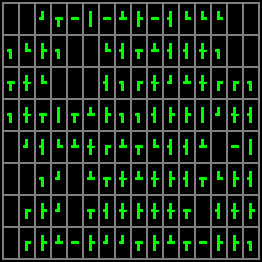
\includegraphics[scale=0.75]{SMT/pipe/shuffled.png}
\caption{Разобранная головоломка}
\end{figure}

\dots и собранная:

\begin{figure}[H]
\label{fig:pipe_solved}
\centering
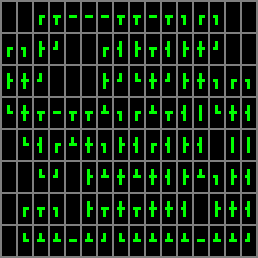
\includegraphics[scale=0.75]{SMT/pipe/solved.png}
\caption{Собранная головоломка}
\end{figure}

Попробуем найти способ собрать её.

\subsubsection{Создание}

В начале, нужно её создать.
Вот простая идея.
Возьем массив ячеек 8*16.
Каждая ячейка может содержать какой-то тип блока.
Между ячейками есть стыки:

\pgfmathsetmacro\Width{16}
\pgfmathsetmacro\Height{8}
%\pgfmathsetmacro\Width{10}
%\pgfmathsetmacro\Height{5}
\pgfmathtruncatemacro\WidthMinusI{\Width - 1}
\pgfmathtruncatemacro\WidthMinusII{\Width - 2}
\pgfmathtruncatemacro\HeightMinusI{\Height - 1}
\pgfmathtruncatemacro\HeightMinusII{\Height - 2}
\pgfmathtruncatemacro\HeightPlusII{\Height + 2}
\pgfmathsetmacro\HeightPlusIi{\Height + 1.5}

% see also: http://www.texample.net/tikz/examples/euclid-algorithm/
\begin{center}
\begin{tikzpicture}[set style={{help lines}+=[dashed]},scale=0.7]

	\draw[style=help lines] (0,0) grid +(\Width,\Height);

	\foreach \c in {0,...,\WidthMinusI}
	{
		\foreach \r in {0,...,\HeightMinusII}
			\draw   [red,very thick,-] (\c+0.5,\r+0.75) -- (\c+0.5,\r+1.25);
		%\node[rotate=90] at (\c+0.5,\HeightPlusII) {\Large vjoints[\dots, \c] \normalsize};
		\node[rotate=90] at (\c+0.5,\HeightPlusII) {vjoints[\dots, \c]};
	}

	\foreach \r in {0,...,\HeightMinusI}
	{
		\foreach \c in {0,...,\WidthMinusII}
			\draw   [blue,very thick,-] (\c+0.75,\r+0.5) -- (\c+1.25,\r+0.5);
		\pgfmathtruncatemacro\hjointslabel{\HeightMinusI - \r}
		%\node at (-1.5,\r+0.5) {\large hjoints[\hjointslabel, \dots] \normalsize};
		\node at (-1.5,\r+0.5) {hjoints[\hjointslabel, \dots]};
	}

\end{tikzpicture}
\end{center}



Синие линии это горизонтальные стыки, красные линии это вертикальные стыки.
Мы просто случайно выставляем каждый стык в 0/false (отсутствует) или 1/true (присутствует).

После этого, теперь легко найти тип каждой ячейки.
А это:

\newcommand{\HeaderColor}{\cellcolor{blue!25}}
\begin{center}
\begin{longtable}{ | l | l | l | l | }
\hline
\HeaderColor стыки & \HeaderColor наше внутреннее название & \HeaderColor угол & \HeaderColor символ \\
\hline
0	&type 0		&	0$^{\circ}$	& (пробел)	\\
2	&type 2a	&	0$^{\circ}$	& \pmboxdrawuni{2503} \\ % ┃
2	&type 2a	&	90$^{\circ}$	& \pmboxdrawuni{2501} \\ % ━
2	&type 2b	&	0$^{\circ}$	& \pmboxdrawuni{250F} \\ % ┏
2	&type 2b	&	90$^{\circ}$	& \pmboxdrawuni{2513} \\ % ┓
2	&type 2b	&	180$^{\circ}$	& \pmboxdrawuni{251B} \\ % ┛
2	&type 2b	&	270$^{\circ}$	& \pmboxdrawuni{2517} \\ % ┗
3	&type 3		&	0$^{\circ}$	& \pmboxdrawuni{2523} \\ % ┣
3 	&type 3		&	90$^{\circ}$	& \pmboxdrawuni{2533} \\ % ┳
3	&type 3		&	180$^{\circ}$	& \pmboxdrawuni{252B} \\ % ┫
3	&type 3		&	270$^{\circ}$	& \pmboxdrawuni{253B} \\ % ┻
4	&type 4		&	0$^{\circ}$	& \pmboxdrawuni{254B} \\ % ╋
\hline
\end{longtable}
\end{center}

\textit{Висящие} стыки могут присутствовать на первой стадии (т.е., ячейки только с одним стыком), но они удалются
рекурсивно, и эти ячейки преобразуются в пустые ячейки.
Так что, в самом конце, все ячейки имеют минимум 2 стыка, и вся эта сантехническая система не имеет связей с внешним миром ---
я надеюсь, из-за этого станет немного проще.

Исходник генератора на Си здесь: \url{https://github.com/DennisYurichev/SAT_SMT_article/tree/master/SMT/pipe/generator}.
Все вертикальные стыки хранятся в глобальном массиве \textit{hjoints[]} и вертикальные в \textit{vjoints[]}.

Программа на Си генерирует ANSI-раскрашенный вывод, как это было показано выше
(\ref{fig:pipe_shuffled}, \ref{fig:pipe_solved}) плюс массив типов для каждой ячейки, но без информации об углах:

\begin{lstlisting}[label=init_cells]
[
["0", "0", "2b", "3", "2a", "2a", "2a", "3", "3", "2a", "3", "2b", "2b", "2b", "0", "0"],
["2b", "2b", "3", "2b", "0", "0", "2b", "3", "3", "3", "3", "3", "4", "2b", "0", "0"],
["3", "4", "2b", "0", "0", "0", "3", "2b", "2b", "4", "2b", "3", "4", "2b", "2b", "2b"],
["2b", "4", "3", "2a", "3", "3", "3", "2b", "2b", "3", "3", "3", "2a", "2b", "4", "3"],
["0", "2b", "3", "2b", "3", "4", "2b", "3", "3", "2b", "3", "3", "3", "0", "2a", "2a"],
["0", "0", "2b", "2b", "0", "3", "3", "4", "3", "4", "3", "3", "3", "2b", "3", "3"],
["0", "2b", "3", "2b", "0", "3", "3", "4", "3", "4", "4", "3", "0", "3", "4", "3"],
["0", "2b", "3", "3", "2a", "3", "2b", "2b", "3", "3", "3", "3", "2a", "3", "3", "2b"],
]
\end{lstlisting}

\subsubsection{Решение}

Прежде всего, мы будем работать с массивом ячеек 8*16, где каждый элемент имеет 4 бита:
``T'' (top/верх),
``B'' (bottom/низ),
``L'' (left/лево),
``R'' (right/право).
Каждый бит представляет собой половину стыка.

% see also: http://www.texample.net/tikz/examples/euclid-algorithm/
\begin{center}
\begin{tikzpicture}[set style={{help lines}+=[dashed]},scale=0.7]

	\draw[style=help lines] (0,0) grid +(\Width,\Height);
	
	\foreach \c in {0,...,\WidthMinusI}
		%\node[rotate=90] at (\c+0.5,\HeightPlusIi) {\Large [\dots, \c] \normalsize};
		\node[rotate=90] at (\c+0.5,\HeightPlusIi) {[\dots, \c]};
	
	\foreach \r in {0,...,\HeightMinusI}
	{
		\pgfmathtruncatemacro\hlabel{\HeightMinusI - \r}
		%\node at (-1.5,\r+0.5) {\large [\hlabel, \dots] \normalsize};
		\node at (-1.5,\r+0.5) {[\hlabel, \dots]};
	
		\pgfmathsetmacro\Shift{0.325}
		\foreach \c in {0,...,\WidthMinusI}
		{
			\node at (\c+0.5,\r+0.5 + \Shift) {\footnotesize T \normalsize};
			\node at (\c+0.5,\r+0.5 - \Shift) {\footnotesize B \normalsize};
			\node at (\c+0.5 - \Shift,\r+0.5) {\footnotesize L \normalsize};
			\node at (\c+0.5 + \Shift,\r+0.5) {\footnotesize R \normalsize};
		}
	}

\end{tikzpicture}
\end{center}


Теперь определяем массив для каждого из четырех полустыков + информация об угле:

\begin{lstlisting}
HEIGHT=8
WIDTH=16

# if T/B/R/L is Bool instead of Int, Z3 solver will work faster
T=[[Bool('cell_%d_%d_top' % (r, c)) for c in range(WIDTH)] for r in range(HEIGHT)]
B=[[Bool('cell_%d_%d_bottom' % (r, c)) for c in range(WIDTH)] for r in range(HEIGHT)]
R=[[Bool('cell_%d_%d_right' % (r, c)) for c in range(WIDTH)] for r in range(HEIGHT)]
L=[[Bool('cell_%d_%d_left' % (r, c)) for c in range(WIDTH)] for r in range(HEIGHT)]
A=[[Int('cell_%d_%d_angle' % (r, c)) for c in range(WIDTH)] for r in range(HEIGHT)]
\end{lstlisting}

Мы знаем, что если каждый из полустыков присутствует, ответный полустык также должен присутствовать, и наоборот. 
Определяем всё это используя эти констрайнты:

\begin{lstlisting}
# shorthand variables for True and False:
t=True
f=False

# "top" of each cell must be equal to "bottom" of the cell above
# "bottom" of each cell must be equal to "top" of the cell below
# "left" of each cell must be equal to "right" of the cell at left
# "right" of each cell must be equal to "left" of the cell at right
for r in range(HEIGHT):
    for c in range(WIDTH):
        if r!=0:
            s.add(T[r][c]==B[r-1][c])
        if r!=HEIGHT-1:
            s.add(B[r][c]==T[r+1][c])
        if c!=0:
            s.add(L[r][c]==R[r][c-1])
        if c!=WIDTH-1:
            s.add(R[r][c]==L[r][c+1])

# "left" of each cell of first column shouldn't have any connection
# so is "right" of each cell of the last column
for r in range(HEIGHT):
    s.add(L[r][0]==f)
    s.add(R[r][WIDTH-1]==f)

# "top" of each cell of the first row shouldn't have any connection
# so is "bottom" of each cell of the last row
for c in range(WIDTH):
    s.add(T[0][c]==f)
    s.add(B[HEIGHT-1][c]==f)
\end{lstlisting}

Теперь перебираем все ячейки в изначальном массиве (\ref{init_cells}).
Первые две ячейки здесь пустые. И третья имеет тип ``2b''.
Это ``\pmboxdrawuni{250F}'' % ┏
и его можно ориентировать четырьмя разными способами.
И если её угол это 0$^{\circ}$, верхний и правый полустыки присутствуют, остальные отсутствуют.
Если он имеет угол 90$^{\circ}$, он выглядит как 
``\pmboxdrawuni{2513}'', % ┓
и верхник и левый полустыки присутствуют, остальные отсутствуют.

На обычном русском языке: ``если ячейка этого типа имеет угол 0$^{\circ}$, вот эти полустыки должны присутствовать \textbf{ИЛИ}
если она имеет угол 90$^{\circ}$, эти полустыки должны присутствовать, \textbf{ИЛИ}, итд, итд.''

Точно также, мы определяем эти правила для всех типов и всех возможных углов:

\begin{lstlisting}
for r in range(HEIGHT):
    for c in range(WIDTH):
        ty=cells_type[r][c]

        if ty=="0":
            s.add(A[r][c]==f)
            s.add(T[r][c]==f, B[r][c]==f, L[r][c]==f, R[r][c]==f)

        if ty=="2a":
            s.add(Or(And(A[r][c]==0, L[r][c]==f, R[r][c]==f, T[r][c]==t, B[r][c]==t),   # §\pmboxdrawuni{2503}§
                    And(A[r][c]==90, L[r][c]==t, R[r][c]==t, T[r][c]==f, B[r][c]==f)))  # §\pmboxdrawuni{2501}§

        if ty=="2b":
            s.add(Or(And(A[r][c]==0, L[r][c]==f, R[r][c]==t, T[r][c]==f, B[r][c]==t),   # §\pmboxdrawuni{250F}§
                    And(A[r][c]==90, L[r][c]==t, R[r][c]==f, T[r][c]==f, B[r][c]==t),   # §\pmboxdrawuni{2513}§
                    And(A[r][c]==180, L[r][c]==t, R[r][c]==f, T[r][c]==t, B[r][c]==f),  # §\pmboxdrawuni{251B}§
                    And(A[r][c]==270, L[r][c]==f, R[r][c]==t, T[r][c]==t, B[r][c]==f))) # §\pmboxdrawuni{2517}§
	
        if ty=="3":
            s.add(Or(And(A[r][c]==0, L[r][c]==f, R[r][c]==t, T[r][c]==t, B[r][c]==t),   # §\pmboxdrawuni{2523}§
                    And(A[r][c]==90, L[r][c]==t, R[r][c]==t, T[r][c]==f, B[r][c]==t),   # §\pmboxdrawuni{2533}§
                    And(A[r][c]==180, L[r][c]==t, R[r][c]==f, T[r][c]==t, B[r][c]==t),  # §\pmboxdrawuni{252B}§
                    And(A[r][c]==270, L[r][c]==t, R[r][c]==t, T[r][c]==t, B[r][c]==f))) # §\pmboxdrawuni{253B}§

        if ty=="4":
            s.add(A[r][c]==0)
            s.add(T[r][c]==t, B[r][c]==t, L[r][c]==t, R[r][c]==t) # §\pmboxdrawuni{254B}§
\end{lstlisting}

Полный исходник здесь: \url{https://github.com/DennisYurichev/SAT_SMT_article/blob/master/SMT/pipe/solver/solve_pipe_puzzle1.py}.

Получается такой результат (выводит угол для каждой ячейки и (псевдо)графическое представление):

\begin{figure}[H]
\centering
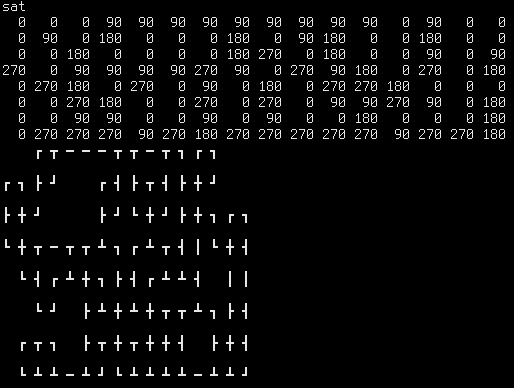
\includegraphics[scale=0.75]{SMT/pipe/solver/solver.png}
\caption{Вывод скрипта солвера}
\end{figure}

Это работает $\approx 4$ секунды на моем старом и медленном Intel Atom N455 1.66GHz.
Быстро ли это? Не знаю, но снова вот что действительно круто, это то что мы понятия не имеем о какой-то математической
теории за всем этим, мы просто объявили ячейки, (полу-)стыки и определили отношения между ними.

Теперь следующий вопрос это, сколько здесь возможных решений?
Используя раннее описанный метод (\ref{SMTEnumerate}), я немного изменил скрипт солвера
\footnote{\url{https://github.com/DennisYurichev/SAT_SMT_article/blob/master/SMT/pipe/solver/solve_pipe_puzzle2.py}} и солвер
сказал что возможно два решения.

Сравним их используя gvimdiff:

\begin{figure}[H]
\centering
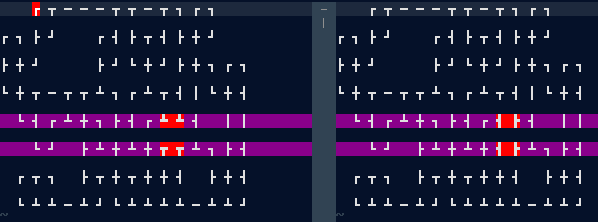
\includegraphics[scale=0.75]{SMT/pipe/solver/diff.png}
\caption{Вывод gvimdiff (извините за мой красный курсор в левой части в левом верхнем углу)}
\end{figure}

4 ячейки в середине могут быть ориентированы по-разному.
Видимо, другие головоломки могут также выдавать разные результаты.

P.S.
\textit{Полу-стык} определен как булевый тип.
Но на самом деле, первая версия солвера была написана используя целочисленный тип для полу-стыков,
и 0 использовалось для False и 1 для True.
Я так сделал, потому что хотел более компактный исходный код, без использования длинных слов как ``False'' и ``True''.
И это работало, но медленнее. Вероятно, Z3 работает с булевыми типами быстрее? Лучше?
Так или иначе, я пишу это чтобы отметить, что, если нужно, целочисленный тип можно использовать вместо булевого.

